\documentclass[english,compress]{beamer}
\usepackage{kloeckislides}
\nonstopmode

\usepackage[normalem]{ulem}
\usepackage{pifont}
\usepackage{ifthen}

\setbeamercolor{section in head/foot}{use=structure,bg=structure.fg!25!bg}
\defbeamertemplate*{footline}{split theme}
{%
  \leavevmode%
  \begin{beamercolorbox}[wd=.5\paperwidth,ht=2.5ex,dp=1.125ex]{section in head/foot}%
    \insertsectionnavigationhorizontal{\paperwidth}{\hskip0pt plus1filll}{}%
  \end{beamercolorbox}%
  %\begin{beamercolorbox}[wd=.5\paperwidth,ht=2.5ex,dp=1.125ex]{subsection in head/foot}%
    %\insertsubsectionnavigationhorizontal{.5\paperwidth}{}{\hskip0pt plus1filll}%
  %\end{beamercolorbox}%
}


%\useoutertheme[subsection=false]{miniframes}

\setbeamertemplate{frametitle}[default][center]

\AtBeginDocument{%
  {
    \usebeamercolor{section in head/foot}
  }
  
  \pgfdeclareverticalshading{beamer@headfade}{\paperwidth}
  {%
    color(0cm)=(bg);
    color(1.25cm)=(section in head/foot.bg)%
  }

  \setbeamercolor{section in head/foot}{bg=}
}

\addtoheadtemplate{\pgfuseshading{beamer@headfade}\vskip-1.25cm}{}

\beamertemplatedotitem

\setbeamercolor{section in head/foot}{parent=palette quaternary}
\setbeamercolor{subsection in head/foot}{parent=palette primary}

\setbeamercolor{author in head/foot}{parent=section in head/foot}
\setbeamercolor{title in head/foot}{parent=subsection in head/foot}



\AtBeginSection[] {
  \begin{frame}<beamer>
  \frametitle{Outline}
  \tableofcontents[sectionstyle=show/shaded,subsectionstyle=show/show/hide]
\end{frame}
}
\AtBeginSubsection[] {
  \begin{frame}<beamer>
  \frametitle{Outline}
  \tableofcontents[sectionstyle=show/shaded,subsectionstyle=show/shaded/hide]
\end{frame}
}

\newcommand{\technicality}[2]{%
  {\strut #1\\
    \begin{beamercolorbox}[sep=1mm]{block body}
      #2
    \end{beamercolorbox}
  }%
}

\lstset{
  language=C++,
  rangebeginprefix=//\ ,
  rangeendprefix=//\ ,
}

\def\weblink#1#2{\href{#1}{\color{blue}\underline{#2}}}

\definecolor{fetch}{RGB}{227,110,35}
\definecolor{alu}{RGB}{255,188,24}
\definecolor{context}{RGB}{132,146,175}

\usepackage{keystroke}

\setbeamertemplate{navigation symbols}{}

\def\hilite<#1>#2{\alt<#1>{\colorbox{blue!30}{#2}}{\colorbox{white}{#2}}%
}

\lstset{
  language=C++,
  rangebeginprefix=/*\ ,
  rangeendprefix=/*\ ,
}

\begin{document}
% {{{ front matter

\title{High-Performance Scientific Computing\\Lecture 11: GPU Performance, Applications}

\date{MATH-GA 2011 / CSCI-GA 2945 $\cdot$ November 21, 2012}

\frame{\titlepage}

\begin{frame}{Today}
  \tableofcontents[hideallsubsections]
\end{frame}
% }}}
% -----------------------------------------------------------------------------
\begin{comment}
\begin{frame}{Bits and pieces}
  \begin{itemize}
    \item Don't have a project? Let's fix that \emph{very soon}
    \item HW5: soon
    \item HW6: due today
    \item Dec 5: Last day of regular class
    \item Dec 12: Legislative Day
    \item Dec 17/18/\textbf{19}: Project presentations
    \item Don't have grade reports for HW1\dots4? Talk to me
  \end{itemize}
\end{frame}
\end{comment}

% -----------------------------------------------------------------------------
\section{GPU performance}
% -----------------------------------------------------------------------------
% {{{
% -----------------------------------------------------------------------------
\subsection{Less control, more data}
% -----------------------------------------------------------------------------
\newcommand{\kayvoncredit}{
  \begin{tikzpicture}[overlay]
    \node [xshift=1cm,yshift=0.5cm]
      at (current page.south west)
      [font=\scriptsize,fill=gray!30,anchor=south west,opacity=0.5]
      {Credit: Kayvon Fatahalian (Stanford) };
  \end{tikzpicture}
}
\newcommand{\kayvonframe}[5]{

  \begin{frame}{#1}
    #4
    \begin{center}
    \includegraphics[viewport=#3,clip=true,page=#2,height=0.7\textheight]{kayvon-gpuarch.pdf}
    \end{center}
    \kayvoncredit
    #5
  \end{frame}
}
\kayvonframe{Gratuitous Amounts of Parallelism!}{24}{5in 1.45in 10in 6.75in }{}{
  \uncover<2->{
    \begin{tikzpicture} [overlay]
      \node [below right=1.75cm of current page.north west, draw,drop shadow,fill=white,
      text width=0.8\textwidth, inner sep=2.5mm,thick]
        {
          Example:

          \medskip
          128 instruction streams in parallel

          16 independent groups of 8 synchronized streams
        } ;
    \end{tikzpicture}
  }
  \uncover<3>{
    \begin{tikzpicture} [overlay]
      \node [above left=1cm of current page.south east, draw,drop shadow,fill=white,
      text width=0.6\textwidth, inner xsep=0.5cm,inner ysep=0.5cm,thick]
        {
          Great if everybody in a group does the same thing.

          \medskip
          But what if not?

          \medskip
          What leads to divergent instruction streams?
        } ;
    \end{tikzpicture}
  }
}
\kayvonframe{Branches}{26}{0.85in 0.9in 10.5in 6.8in }{}{}
\kayvonframe{Branches}{27}{0.85in 0.9in 10.5in 6.8in }{}{}
\kayvonframe{Branches}{28}{0.85in 0.9in 10.5in 6.8in }{}{}
\kayvonframe{Branches}{29}{0.85in 0.9in 10.5in 6.8in }{}{}
% -----------------------------------------------------------------------------
\begin{frame}{GPUs vs Branching}
  \begin{center}
  \Huge Branch demo time
  \end{center}
\end{frame}
% -----------------------------------------------------------------------------
\subsection{GPUs and Latency}
% -----------------------------------------------------------------------------
\begin{frame}{GPUs vs Latency}
  \begin{columns}
    \column{0.6\textwidth}
      \begin{block}{Problem}
        Memory still has very high latency\dots

        \dots as do many other things\dots

        \dots but we've removed most of the hardware that helps us
        deal with that.

      \end{block}
      \medskip
      We've removed
      \begin{itemize}
      \item caches
      \item branch prediction
      \item out-of-order execution
      \end{itemize}

      So what now?
    \column{0.4\textwidth}
      \includegraphics[width=\textwidth]{memory.png}
  \end{columns}
  \uncover<2->{
    \begin{tikzpicture} [overlay]
      \node [below right=1cm of current page.north west, draw,drop shadow,fill=white,
      text width=0.6\textwidth, inner sep=5mm,thick]
      {
        \only<2-3>{\includegraphics[viewport=6.25in 1in 10.25in 4.75in,clip=true,page=33,width=\textwidth]{kayvon-gpuarch.pdf}}%
        \only<4>{\includegraphics[viewport=6.25in 1in 10.25in 4.75in,clip=true,page=34,width=\textwidth]{kayvon-gpuarch.pdf}}%
      };
    \end{tikzpicture}
  }
  \uncover<3->{
    \begin{tikzpicture} [overlay]
      \node [above left=1cm of current page.south east, draw,drop shadow,fill=white,
      text width=0.4\textwidth, inner sep=5mm,thick]
      {
        \textbf{Idea \#3}

        \medskip
        \begin{tabular}{rl}
        & Even more parallelism \\ + &Some extra memory \\ \hline = &A solution!
        \end{tabular}

      };
    \end{tikzpicture}
  }
\end{frame}

\kayvonframe{Hiding Memory Latency}{33}{0.65in 0.85in 10.4in 6.8in }{}{}
\kayvonframe{Hiding Memory Latency}{34}{0.65in 0.85in 10.4in 6.8in }{}{}
\kayvonframe{Hiding Memory Latency}{35}{0.65in 0.85in 10.4in 6.8in }{}{}
\kayvonframe{Hiding Memory Latency}{36}{0.65in 0.85in 10.4in 6.8in }{}{}
\kayvonframe{Hiding Memory Latency}{37}{0.65in 0.85in 10.4in 6.8in }{}{}
\kayvonframe{Hiding Memory Latency}{38}{0.65in 0.85in 10.4in 6.8in }{}{}

% -----------------------------------------------------------------------------
\begin{frame}{Architecture}
  \begin{center}
  \Huge GPUs and latency demo
  \end{center}
\end{frame}
% -----------------------------------------------------------------------------
\subsection{Understanding GPUs}
% -----------------------------------------------------------------------------
\begin{frame}{Comparing architectures}
  \begin{tabular}{l|cccc|l}
    & GF100 & GF104 & GK104 & GCN & Units\\
    \hline
    \# Warps/Wavefronts & 48 & 48 & 64 & 40 \\
    Warp Size & 32 & 32 & 32 & 64 & W.Item \\
    \hline
    SP FLOP/clock & 64 & 96 & 384 & 128 \\
    Clock & 700 & 650 & 823 & 925 & MHz \\
    \hline
    Reg File & 128 & 128 & 256 & 256 & kiB \\
    Lmem & 64  & 64 & 64 & 64 & kiB \\
    Lmem BW & 64  & 64 & 128 & 128 & B/clock \\
    \hline
  \end{tabular}
  \creditto{David Kanter / Realworldtech.com}
\end{frame}
% -----------------------------------------------------------------------------
\begin{frame}{Architecture}
  \begin{center}
  \Huge Architecture by the numbers demo
  \end{center}
\end{frame}
% -----------------------------------------------------------------------------
\begin{frame}{Architecture}
  \begin{center}
  \Huge Occupancy calculator
  \end{center}
\end{frame}
% -----------------------------------------------------------------------------
\subsection{GPUs and Memory}
% -----------------------------------------------------------------------------
\input{parallel-memories}
\input{cl-gmem-access}
% -----------------------------------------------------------------------------
\begin{frame}{GPU Global Memory}
  \begin{center}
  \Huge GPU global access patterns demo
  \end{center}
\end{frame}
% -----------------------------------------------------------------------------
\input{cl-lmem-access}
% -----------------------------------------------------------------------------
\begin{frame}{GPU local Memory}
  \begin{center}
  \Huge GPU local access patterns demo
  \end{center}
  \uncover<+->{}
  \uncover<+->{
    \begin{tikzpicture} [overlay]
      \node [above left=1cm of current page.south east,draw,drop shadow,fill=white,
       inner sep=5mm,thick,text width=0.6\textwidth]
        {
          What does this mean for 2D arrays in local memory? (E.g. matrix transpose?)

          \only<+->{
            \bigskip
            What does this mean for \texttt{double}s in local memory?
          }
        } ;
    \end{tikzpicture}
  }
\end{frame}
% -----------------------------------------------------------------------------
{
  \newcommand{\brick}[6]{
    \draw [fill=#4!50]
      (0,0) rectangle (#1,#2) coordinate [pos=0.5] (brickfront);
    \draw [fill=#4]
      (#1,0) -- (#1,0,-1) -- (#1,#2,-1) -- (#1,#2) --cycle;
    \draw [fill=#4]
      (0,#2) -- (0,#2,-1) -- (#1,#2,-1) -- (#1,#2) --cycle;
    #6
    \begin{pgfonlayer}{foreground}
      \node [fill=#4!50,inner xsep=2pt,inner ysep=2pt,opacity=0.7,#5] at (brickfront) { #3 } ;
      \node [#5] at (brickfront) { #3 } ;
    \end{pgfonlayer}
  }
  \newcommand{\drawevt}[2]{
    \fill [#2,opacity=0.5] 
      (0,#1) -- (1.5,#1) -- (1.5,#1,-1)
      -- (1.5,#1+0.2,-1) -- (1.5,#1+0.2) -- (0,#1+0.2) --  cycle ;
  }
  \begin{frame}{Faster transfers Host $\leftrightarrow$ GPU}
    \begin{columns}
      \column{0.55\textwidth}
        How about host $\leftrightarrow$ device transfers?
        \begin{itemize}
          \item If talking to CPU: Unnecessary
            \uncover<2->{\texttt{CL\_MEM\_ALLOC\_HOST\_PTR}}
          \item If talking to GPU:

            \medskip
            \begin{itemize}
              \item Want asynchronous transfer
              \item Want overlapping transfer
            \end{itemize}

            \medskip
            What about paging?

            \uncover<3->{
              \texttt{CL\_MEM\_ALLOC\_HOST\_PTR}

              \medskip
              (`pinned' memory--Demo)
            }
        \end{itemize}

      \column{0.4\textwidth}
        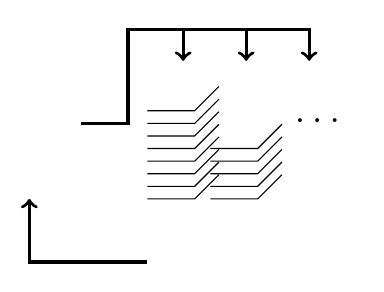
\begin{tikzpicture}[scale=0.8]
          \brick{1.25}{2}{Host}{gray}{}{}
          \begin{scope}[xshift=2.5cm,yshift=-1.5cm]
            \brick{2.5}{1.25}{Device}{gray}{}{}
          \end{scope}
          \begin{scope}[xshift=2.5cm]
            \brick{0.75}{2}{Queue 1}{blue}{text=white,rotate=90}{
              \foreach\i in {0,0.2,...,1.4}
                \draw (0,\i) -- (0.75,\i) -- (0.75,\i,-1);
            }
          \end{scope}
          \begin{scope}[xshift=3.5cm]
            \brick{0.75}{2}{Queue 2}{blue}{text=white,rotate=90}{
              \foreach\i in {0,0.2,...,0.9}
                \draw (0,\i) -- (0.75,\i) -- (0.75,\i,-1);
            }
          \end{scope}

          \node [font=\Large] at (5.25,1.25) {\dots} ;

          \draw [very thick,->] (1.25,1,-0.5) -| (2,2.5,-0.5) -| (2.875,2,-0.5);
          \draw [very thick,->] (2,2.5,-0.5) -| (3.875,2,-0.5);
          \draw [very thick,->] (2,2.5,-0.5) -| (4.875,2,-0.5);
          \draw [very thick,->] (2.5,-1) -| (0.625,0);
        \end{tikzpicture}
    \end{columns}
  \uncover<4->{
    \begin{tikzpicture} [overlay]
      \node [above left=1cm of current page.south east,draw,drop shadow,fill=white,
       inner sep=5mm,thick, text width=0.6\textwidth]
        {
          Important: Two different mechanisms at work!
        } ;
    \end{tikzpicture}
  }
  \end{frame}
}
% -----------------------------------------------------------------------------
\begin{frame}{Entertainment: GPU Memory Zoo}

  \uncover<+->{
    \begin{tabular}{p{5em}cccp{2.8cm}}
    \hline
    \textbf{Type} & \textbf{Per} & \textbf{Access} & \textbf{Latency} \\
    \hline
    \textbf<2->{private} & work item & R/W & 1 or 1000 \\
    \textbf<2->{local} & group & R/W & 2 \\
    \textbf<2->{global} & grid & R/W & 1000 & Cached?\\
    \texttt{constant} & grid & R/O & 1-1000 & Cached \\
    image$n$d\_t & grid & R(/W) & 1000 & Spatially cached\\
    \hline
    \end{tabular}
  }
\end{frame}
% -----------------------------------------------------------------------------
\subsection{Summary}
% -----------------------------------------------------------------------------
\begin{frame}{GPU performance summary}
  \begin{itemize}
    \item Latency, latency, latency!
      \begin{itemize}
        \item Various forms: Memory, branches, computation
        \item All need to be hidden
      \end{itemize}
    \item Bandwidth: usually fixable
    \item Watch your memory access patterns
      \begin{itemize}
        \item Local mem is somewhat more forgiving
        \item \dots and lower latency, higher BW
      \end{itemize}
  \end{itemize}
\end{frame}
\begin{frame}{Demo}
  \begin{center}
  \Huge GPU profiler demo
  \end{center}
\end{frame}

% }}}
% -----------------------------------------------------------------------------
\section{MPI performance}
% -----------------------------------------------------------------------------
\begin{frame}{MPI}
  \begin{center}
  \Huge MPI performance demo
  \end{center}
\end{frame}

% {{{

% TODO:
% - pinned memory
% - MPI performance

% case study: optimize mat-mat

% }}}
\questionframe{}
%\imagecreditslide

\end{document}
